\chapter{Opis projektnog zadatka}
		
		%\textbf{\textit{dio 1. revizije}}\\
		
		%\textit{Na osnovi projektnog zadatka detaljno opisati korisničke zahtjeve. Što jasnije opisati cilj projektnog zadatka, razraditi problematiku zadatka, dodati nove aspekte problema i potencijalnih rješenja. Očekuje se minimalno 3, a poželjno 4-5 stranica opisa.	Teme koje treba dodatno razraditi u ovom poglavlju su:}
		%\begin{packed_item}
		%	\item \textit{potencijalna korist ovog projekta}
		%	\item \textit{postojeća slična rješenja (istražiti i ukratko opisati razlike u odnosu na zadani zadatak). Dodajte slike koja predočavaju slična rješenja.}
		%	\item \textit{skup korisnika koji bi mogao biti zainteresiran za ostvareno rješenje.}
		%	\item \textit{mogućnost prilagodbe rješenja }
		%	\item \textit{opseg projektnog zadatka}
		%	\item \textit{moguće nadogradnje projektnog zadatka}
		%\end{packed_item}
		
		%\textit{Za pomoć pogledati reference navedene u poglavlju „Popis literature“, a po potrebi konzultirati sadržaj na internetu koji nudi dobre smjernice u tom pogledu.}
		%\eject
		
		U današnje vrijeme veliki broj ljudi za svog ljubimca odabire psa, koji većinu vremena provodi uz svog vlasnika. No, što ako vlasnik ima neodgodivu obavezu na koju nikako ne može povesti svog psa i treba biti odsutan neko vrijeme? Kome se obratiti za pomoć, ako mu je nitko koga zna nije u mogućnosti ponuditi? Negdje u blizini se sigurno krije osoba koja bi rado preuzela privremenu brigu, no kako do nje? 
		
		Kako bi vlasnici mogli obavljati svoje obaveze bezbrižno znajući da je njihov pas zbrinut, a s druge strane ljudi koji bi rado prošetali ili nahranili psa i privremeno se igrali s njim mogli ispuniti vrijeme na koristan i zabavan način, potrebna je aplikacija preko koje bi se oni mogli povezati i pronaći rješenje za svoje brige. 
		
		Glavni cilj ovog projekta je stvaranje aplikacije \textit{"Čuvari pasa"} koja će vlasniku pasa pomoći u pronalasku osobe koja najbolje odgovara za privremenu brigu (od nekoliko sati do nekoliko tjedana ili mjeseci) o njegovom ljubimcu. 
		
		Ukratko, ideja je da vlasnik pasa u aplikaciji predaje zahtjev kojim traži osobu za privremenu brigu o njegovom psu. S druge strane, osobe koje su voljne čuvati nekog psa na određeno vrijeme u aplikaciji predaju oglas u kojem navode uvjete čuvanja/brige. Na temelju zahtjeva vlasnika i uvjeta čuvara, aplikacija može prona-ći najbolji odabir, koji su obje strane u mogućnosti prihvatiti ili odbiti, pa u slučaju odbijanja pretražujući  ostale zahtjeve/oglase pronaći drugi odabir. 
		
		Prilikom pokretanja aplikacije prikazuje se početna stranica na kojoj se nalazi nekoliko informacija o samoj aplikaciji te navigacijski izbornik putem kojeg se može pristupiti registraciji i prijavi u sustav te objavljenim zahtjevima i oglasima. Pregledavanje tih zahtjeva i oglasa omogućeno je i neregistriranim korisnicima, ali za korištenje ostalih funkcionalnosti, kao što su objava vlastitih zahtjeva/oglasa te stupanje u kontakt s objavljivačima, potrebna je registracija ili u slučaju već postojećeg računa, prijava. Registrirati se može bilo tko na način da unese osnovne podatke koji su potrebni za korištenje aplikacije, a to su: ime, prezime, korisničko ime, e-mail adresa, lozinka i uloga (\textit{vlasnik/čuvar/oboje}). 
		
		S druge strane, korisnik koji je već registriran može se prijaviti u sustav unoseći korisničko ime i lozinku. Registracijom u sustav korisniku se dodjeljuje odabrana uloga (\textit{vlasnik/čuvar/oboje}). On u tom slučaju može pregledavati svoje osobne podatke te se odjaviti iz sustava, a u nastavku su opisane funkcionalnosti i mogućnosti za pojedinu ulogu korisnika. 
		
		\textit{Korisnik (vlasnik pasa):}
		
		U slučaju da je korisnik odabrao ulogu vlasnika pasa, on ima mogućnost kreiranja zahtjeva za čuvanje pasa u aplikaciji. Pri kreiranju zahtjeva potrebno je unijeti osnovne podatke vezane za čuvanje, a to su: potrebni period čuvanja, potrebne aktivnosti (npr. šetnja, istrčavanje, hranjenje – potrebna količina hrane ako se radi o hranjenju itd.), lokacija čuvanja te željene karakteristike potencijalnog čuvara (ima li čuvar iskustva u čuvanju te ima li vlastitog psa). Osim osnovnih podataka, vlasnik iz liste vlastitih pasa može odabrati pse koje je potrebno čuvati. Svoje pse vlasnik može dodavati na posebnoj stranici i pritom mora unijeti ime psa, datum rođenja i objaviti sliku svog psa. Sve zahtjeve koje je korisnik kreirao može pregledati na zasebnoj stranici za prikaz vlastitih stvorenih zahtjeva. Također, korisnik putem zaglavlja ima mogućnost pregleda svih oglasa koje su objavili čuvari pasa i svih zahtjeva koje su objavili drugi vlasnici pasa.
		
		\textit{Korisnik (čuvar pasa):}
		
		U slučaju da je korisnik odabrao ulogu čuvara pasa, on ima mogućnost kreiranja oglasa u aplikaciji kojim nudi uslugu čuvanja. Pri kreiranju oglasa potrebno je unijeti osnovne podatke relevantne za oglas, a to su: pasmina koju želi čuvati, preferirana dob pasa, mogući period čuvanja (te je li period fiksan ili fleksibilan), lokacija i željeni broj pasa za čuvanje. Sve oglase koje je korisnik kreirao može pregledati na zasebnoj stranici za prikaz vlastitih stvorenih oglasa. Također, korisnik putem zaglavlja ima mogućnost pregleda svih zahtjeva koje su objavili vlasnici pasa i svih oglasa koje su objavili drugi čuvari pasa.
		
		Uz ulogu korisnika, postoji i uloga administratora.
		
		\textit{Administrator} sustava, uz funkcionalnosti ranije opisanih korisnika, ima i neke dodatne mogućnosti kao što su: upravljanje zahtjevima/oglasima koje su kreirali vlasnik/čuvar pasa, blokiranje korisnika koji narušavaju pravila sustava te dodjeljivanje administratorskih ovlasti drugom korisniku. Osobni podaci registriranog korisnika bit će vidljivi samo administratoru i koristit će se u svrhu ostvarenja kontakta između uparenih vlasnika i čuvara pasa. Prije javne objave bilo kojeg zahtjeva/oglasa, on se šalje administratoru na uvid u posebnoj kartici koja je vidljiva samo korisnicima s administratorskim ovlastima u aplikaciji, a koji potom odlučuje hoće li taj zahtjev/oglas biti javno dostupan.
		
		Nakon što administrator odobri stvoreni zahtjev/oglas, on postaje javno dostupan te potom korisnik ima dvije mogućnosti za pronalazak najboljeg odgovarajućeg čuvara pasa/psa za čuvanje:
		
		\begin{packed_item}
			
			\item Odabir \textit{"Najbolja ponuda"} kojim aplikacija na temelju pojedinih karakteristika (pasmina, dob psa, period čuvanja, udaljenost lokacija vlasnika i čuvara) pronalazi najpogodnijeg čuvara/psa. Ukoliko se pronađe takav zahtjev/oglas te korisnik koji je inicirao ovu opciju odluči prihvatiti pronađenu ponudu, korisniku čiji je zahtjev/oglas bio ponuđen, u aplikaciji se pojavljuje zahtjev/oglas za koji je odabrana opcija najbolje ponude na stranici za pregled pristiglih ponuda. Korisnici imaju mogućnost prihvaćanja pristigle ponude i ako oba korisnika prihvate odabir tada im se na pregledu trenutnih čuvanja prikazuje i kontakt drugog korisnika te se mogu dogovoriti za detalje. Ako barem jedan korisnik odbije odabir, tada se smatra da nije poželjna daljnja suradnja.
			\item Korisnik ručno pregledava sve zahtjeve/oglase u aplikaciji, pronalazi onaj koji mu se najviše sviđa i odabirom javljanja na istog šalje čuvaru/vlasniku pasa taj zahtjev/oglas u pristigle ponude čime se daje do znanja da je zainteresiran za suradnju. Čuvar/vlasnik pasa taj odabir prihvaća te se potom na stranici trenutnih čuvanja prikazuje kontakt za daljnji dogovor oko detalja, ili odbija što bi značilo da jedna od strana ne želi ostvariti suradnju.
			
		\end{packed_item}
		
		Nakon završene suradnje  vlasnik pasa može ocijeniti koliko je zadovoljan uslugom čuvanja. S druge strane, čuvar pasa isto tako može ocijeniti kakav je bio pas za čuvanje. Prosječna ocjena kojom je ocjenjen čuvar pasa služi tome da bi vlasnik pasa mogao na temelju tuđih mišljenja procijeniti je li baš taj čuvar pogodan za njegovog ljubimca. Isto tako, prosječna ocjena psa služi tome da bi potencijalni čuvar mogao procjeniti je li taj pas pogodan za čuvanje na temelju tuđih iskustava.
		
		Aplikacija treba biti izvedena kao web aplikacija prilagođena mobilnom uređaju i tabletu kojoj će registrirani korisnici pristupati uz pomoć korisničkog imena i lozinke. Također, sustav treba podržavati rad više korisnika u stvarnom vremenu.\newline
		
		
		
		Aplikacija ima puno prostora za nadogradnju u budućnosti. Neke od početnih ideja nadogradnje bile bi 
		dodavanje mogućnosti pregledavanja korisničkih računa drugih korisnika (uz to bi se i nadogradile mogućnosti uređivanja samog korisnič-kog računa - npr. moguće objavljivanje fotografija svojih ljubimaca) i slanja zahtjeva za prijateljstvo, kako bi osobe mogle ostati povezane za potencijalnu buduću suradnju. Također, moguće proširenje aplikacije bila bi implementacija sustava kojim se oglašavaju psi za udomljvanje i zbrinjavanje.\newline
		
		Neke funkcionalnosti ove aplikacije mogle bi se usporediti s funkcionalnostima aplikacije za pružanje usluga prijevoza pod nazivom \textit{"Uber"}. Aplikacija \textit{"Uber"} ima funkcionalnost pronalaska najboljeg odabira, koja radi na način da uparuje vozače i korisnike s najpogodnijom lokacijskom udaljenosti, tako da korisniku u što kraćem roku bude pružena željena usluga. Po završetku vožnje korisnik također ima opciju ocijeniti koliko je bio zadovoljan vožnjom. Navedene funkcionalnosti su vrlo slične funkcionalnostima aplikacije kojom se bavi ovaj projekt.
		%ostatak teksta je zakomentiran
		\iffalse
		\section{Primjeri u \LaTeX u}
		
		\textit{Ovo potpoglavlje izbrisati.}\\

		U nastavku se nalaze različiti primjeri kako koristiti osnovne funkcionalnosti \LaTeX a koje su potrebne za izradu dokumentacije. Za dodatnu pomoć obratiti se asistentu na projektu ili potražiti upute na sljedećim web sjedištima:
		\begin{itemize}
			\item Upute za izradu diplomskog rada u \LaTeX u - \url{https://www.fer.unizg.hr/_download/repository/LaTeX-upute.pdf}
			\item \LaTeX\ projekt - \url{https://www.latex-project.org/help/}
			\item StackExchange za Tex - \url{https://tex.stackexchange.com/}\\
		
		\end{itemize} 	


		
		\noindent \underbar{podcrtani tekst}, \textbf{podebljani tekst}, 	\textit{nagnuti tekst}\\
		\noindent \normalsize primjer \large primjer \Large primjer \LARGE {primjer} \huge {primjer} \Huge primjer \normalsize
				
		\begin{packed_item}
			
			\item  primjer
			\item  primjer
			\item  primjer
			\item[] \begin{packed_enum}
				\item primjer
				\item[] \begin{packed_enum}
					\item[1.a] primjer
					\item[b] primjer
				\end{packed_enum}
				\item primjer
			\end{packed_enum}
			
		\end{packed_item}
		
		\noindent primjer url-a: \url{https://www.fer.unizg.hr/predmet/proinz/projekt}
		
		\noindent posebni znakovi: \# \$ \% \& \{ \} \_ 
		$|$ $<$ $>$ 
		\^{} 
		\~{} 
		$\backslash$ 
		
		
		\begin{longtblr}[
			label=none,
			entry=none
			]{
				width = \textwidth,
				colspec={|X[8,l]|X[8, l]|X[16, l]|}, 
				rowhead = 1,
			} %definicija širine tablice, širine stupaca, poravnanje i broja redaka naslova tablice
			\hline \multicolumn{3}{|c|}{\textbf{naslov unutar tablice}}	 \\ \hline[3pt]
			\SetCell{LightGreen}IDKorisnik & INT	&  	Lorem ipsum dolor sit amet, consectetur adipiscing elit, sed do eiusmod  	\\ \hline
			korisnickoIme	& VARCHAR &   	\\ \hline 
			email & VARCHAR &   \\ \hline 
			ime & VARCHAR	&  		\\ \hline 
			\SetCell{LightBlue} primjer	& VARCHAR &   	\\ \hline 
		\end{longtblr}
		

		\begin{longtblr}[
				caption = {Naslov s referencom izvan tablice},
				entry = {Short Caption},
			]{
				width = \textwidth, 
				colspec = {|X[8,l]|X[8,l]|X[16,l]|}, 
				rowhead = 1,
			}
			\hline
			\SetCell{LightGreen}IDKorisnik & INT	&  	Lorem ipsum dolor sit amet, consectetur adipiscing elit, sed do eiusmod  	\\ \hline
			korisnickoIme	& VARCHAR &   	\\ \hline 
			email & VARCHAR &   \\ \hline 
			ime & VARCHAR	&  		\\ \hline 
			\SetCell{LightBlue} primjer	& VARCHAR &   	\\ \hline 
		\end{longtblr}
	


		
		
		%unos slike
		\begin{figure}[H]
			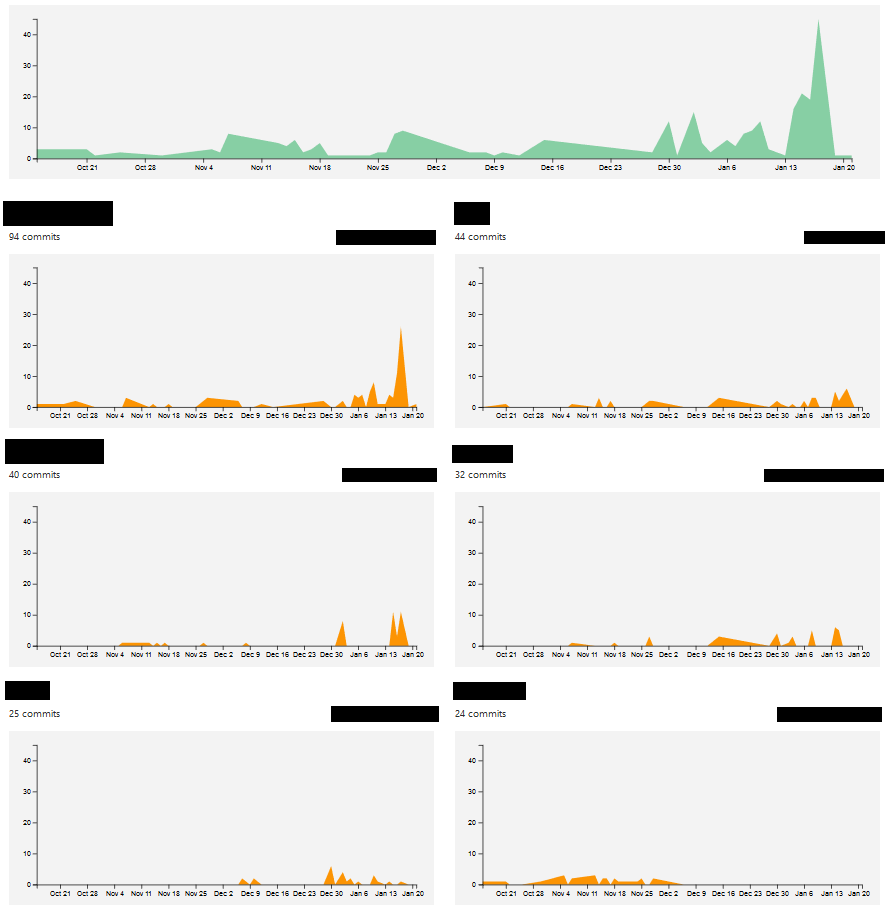
\includegraphics[scale=0.4]{slike/aktivnost.PNG} %veličina slike u odnosu na originalnu datoteku i pozicija slike
			\centering
			\caption{Primjer slike s potpisom}
			\label{fig:promjene}
		\end{figure}
		
		\begin{figure}[H]
			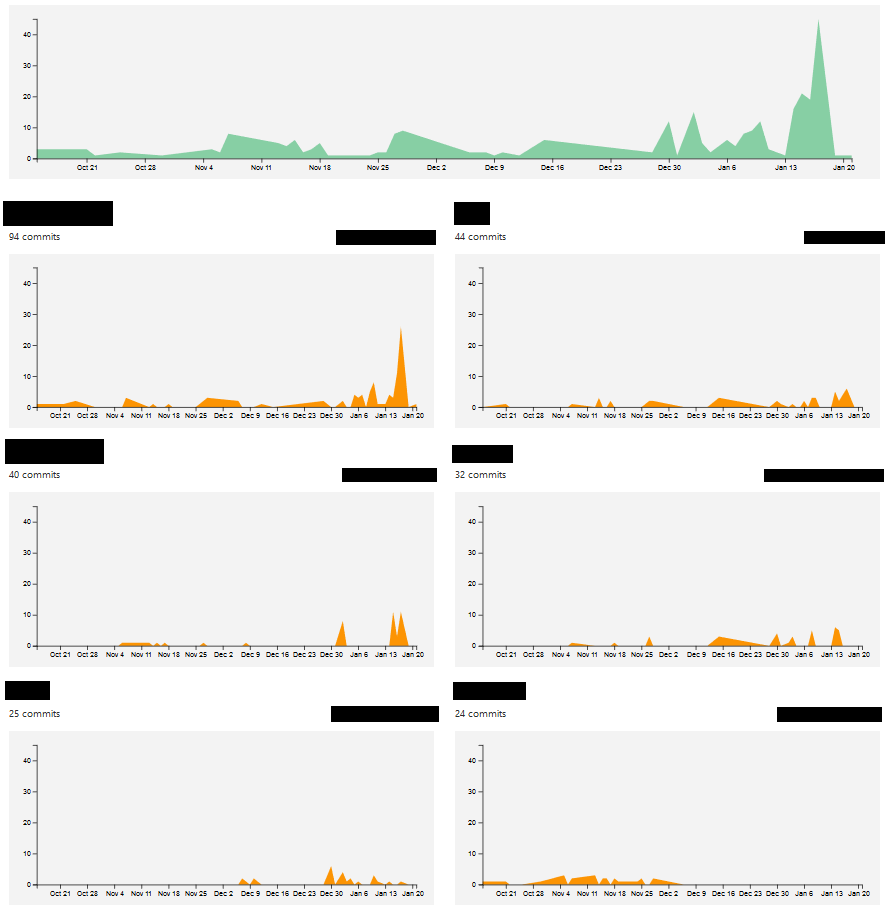
\includegraphics[width=\textwidth]{slike/aktivnost.PNG} %veličina u odnosu na širinu linije
			\caption{Primjer slike s potpisom 2}
			\label{fig:promjene2} %label mora biti drugaciji za svaku sliku
		\end{figure}
		
		Referenciranje slike \ref{fig:promjene2} u tekstu.
		
		\eject
		\fi
	